\documentclass[12pt,a4paper]{article}
\usepackage[utf8]{inputenc}
\usepackage{amsmath,amssymb,amsthm}
\usepackage{geometry}
\usepackage{setspace}
\usepackage[hidelinks]{hyperref}
\usepackage{natbib}
\usepackage{graphicx}
\usepackage{booktabs}
\usepackage{caption}
\geometry{margin=1in}
\onehalfspacing

\newtheorem{definition}{Definition}
\newtheorem{lemma}{Lemma}
\newtheorem{proposition}{Proposition}
\newtheorem{theorem}{Theorem}
\newtheorem{remark}{Remark}
\newtheorem{corollary}{Corollary}
\newtheorem{assumption}{Assumption}

\title{Cherry-Picking under Screening:\\
  Selective Disclosure and Participation in
  Pharmaceutical Approval}
\author{Xueyang}
\date{March 2026}

\begin{document}
\maketitle


% ============================================================
\section{Introduction}
\label{sec:intro}
% ============================================================

A central challenge in pharmaceutical regulation is that the
firm conducting a clinical trial has better information about
the trial's outcome than the regulator evaluating the drug.
This information asymmetry creates scope for
\emph{cherry-picking}: the firm selectively discloses
favorable results while suppressing unfavorable ones. A
growing empirical literature documents this phenomenon. For
instance, \citet{turner2008} show that among 74 FDA-registered
antidepressant trials, 94\% of published trials reported
positive results, compared to only 51\% of all registered
trials---a discrepancy driven by selective publication. More
recently, \citet{deangelis2004} and
\citet{alltrials2013} have called for mandatory registration
and disclosure of all trial results.

Despite this empirical salience, the theoretical literature on
pharmaceutical approval has largely assumed full transparency.
\citet{min2023} studies a screening problem where the FDA
observes both the experiment chosen by the firm and its
outcome, designing approval probabilities to screen
heterogeneous firm types. The present paper extends Min's
framework in two directions, each motivated by real-world
features of drug development.

The first modification is \emph{voluntary disclosure}: the
firm chooses whether to include trial evidence in its drug
application. If disclosed, the FDA observes verified evidence
$(\pi, j)$; if omitted, the FDA sees only an application
without supporting data ($\emptyset$). This creates a pooling
problem, because the FDA must set a single approval
probability $A(\emptyset)$ for all no-evidence applications,
regardless of the underlying type or outcome. From the FDA's
perspective, an application without evidence is
informationally ambiguous---it could reflect a suppressed
negative result, an ongoing trial with no conclusion yet, or
inconclusive preliminary data. This ambiguity is not merely a
modeling artifact; it corresponds directly to regulatory
reality. The FDA's accelerated approval
pathway\footnote{21 CFR Part 314, Subpart H. See
\url{https://www.ecfr.gov/current/title-21/chapter-I/subchapter-D/part-314/subpart-H}.}
grants approval based on surrogate endpoints or limited
evidence, with post-market confirmatory studies required.
Emergency Use Authorizations\footnote{Section 564 of the
Federal Food, Drug, and Cosmetic Act. See
\url{https://www.fda.gov/emergency-preparedness-and-response/mcm-legal-regulatory-and-policy-framework/emergency-use-authorization}.}
similarly allow approval before full trials are complete. In each case, the
regulator commits to a positive approval probability for
applications that lack definitive trial evidence---precisely
the $A(\emptyset) > 0$ that emerges endogenously in my model.

The second modification is \emph{costly participation}: drug
development requires a fixed cost $c > 0$ before any
experiment can be run. If the expected payoff from the
approval mechanism is too low, the firm does not develop, and
no drug exists for the FDA to evaluate. This introduces an
individual rationality (IR) constraint absent from Min's
model.

The model is a standard screening problem in the tradition of
\citet{maskinriley1984} and \citet{mussarosen1978}. The FDA
(principal) designs a menu of contracts---here, pairs of
experiments and approval probabilities---to screen the firm's
(agent's) private type. The analysis relies on three
canonical tools: incentive compatibility (IC), which ensures
each type prefers its assigned contract; individual
rationality (IR), which ensures each type prefers
participation to non-participation; and the revelation
principle, which guarantees that restricting attention to
direct, truthful mechanisms is without loss of generality.
The novel feature relative to the textbook screening problem
is the \emph{pooling constraint}: the silence channel
$A(\emptyset)$ is shared across all types, unlike the
type-specific bad-result probabilities $A_b^i$ available
under Min's full-transparency regime.

The paper delivers four main results. First,
Theorem~\ref{thm:no_IR} shows that without participation
constraints, the FDA's optimal committed mechanism sets
$A(\emptyset) = 0$: the disclosure option is
payoff-irrelevant and the solution reduces exactly to
\citet{min2023}. Second, Theorem~\ref{thm:with_IR}
establishes that when the IR constraint binds, the FDA may
optimally set $A(\emptyset) > 0$ to induce participation,
with a closed-form threshold
$\alpha^* = (c - h_2)/(1 - h_2)$. This positive approval
probability for no-evidence applications is not regulatory
negligence; it is a rational design choice in which the FDA
accepts a higher risk of approving bad drugs in exchange for
ensuring that good drugs get developed.  Third,
Corollary~\ref{cor:welfare} quantifies the welfare cost of
pooling: participation-inducing is strictly more costly under
voluntary disclosure than under full transparency, and the
welfare difference $t|\Delta_b(\pi_1)|\alpha^*$ measures the
price of cherry-picking. Fourth,
Proposition~\ref{prop:both_IC} extends the analysis to
overlapping feasible sets where both IC constraints bind,
deriving a semi-closed-form solution in which the big type's
approval probability is distorted downward---a reversed
screening distortion relative to the standard
\citet{maskinriley1984} result---and validating it
numerically.


% ============================================================
\section{Model Setup}
\label{sec:model}
% ============================================================

\subsection{Primitives}

Two players: a pharmaceutical firm (the agent, ``he'') and
the FDA (the principal, ``she'').

\paragraph{States and prior.}
$\omega \in \{G, B\}$, with
$\Pr(G) = p \in (0, 1/2)$.

\paragraph{Payoffs.}
The FDA receives 1 for a correct decision and 0 otherwise.
The firm cares only about approval:
$U_A(A, \cdot) = 1$, $U_A(D, \cdot) = 0$.

\paragraph{Development cost.}
Before running any experiment, the firm incurs a development
cost $c > 0$. If the firm does not develop, no drug exists
and the FDA makes no decision. The FDA's payoff from
non-participation equals $1 - p$: since $p < 1/2$, the prior
favors rejection, and the expected payoff from no drug on the
market is $\Pr(B) \cdot 1 + \Pr(G) \cdot 0 = 1 - p$.

\begin{remark}[Role of $c$]
In \citet{min2023}, the firm always participates
($c = 0$ implicitly). With $c > 0$, the firm's individual
rationality constraint can bind, creating a force for
$A(\emptyset) > 0$ absent from Min.
\end{remark}


\subsection{Types and Feasible Sets}

The firm has a privately known type
$\theta_i \in \{\theta_1, \theta_2\}$, with
$\Pr(\theta_1) = t$. Type determines the set of feasible
experiments $S_i$.

\begin{assumption}[Feasible sets]\label{as:feasible}
$S_2 \subset S_1$, and both satisfy:
\begin{enumerate}
  \item[(i)] Each $S_i$ is a closed, convex subset of
    $\{(x, y) \in [0,1]^2 : y \geq 1 - x\}$.
  \item[(ii)] The upper boundary
    $\bar{S}_i(x) := \max\{y : (x,y) \in S_i\}$ is
    continuous, concave, and strictly decreasing.
\end{enumerate}
\end{assumption}

Here $\theta_1$ is the ``big type'' (larger feasible set)
and $\theta_2$ is the ``small type.''


\subsection{Experiments}

An experiment $\pi = (x, y) \in S_i$ produces a binary outcome
$j \in \{g, b\}$:
\[
  \Pr(g \mid G, \pi) = y, \quad
  \Pr(g \mid B, \pi) = 1 - x.
\]
An experiment is \emph{convincing} if
$py \geq (1 - p)(1 - x)$.


\subsection{Disclosure and Information Structure}
\label{sec:modification}

After observing the trial outcome $j$, the firm submits a
drug application to the FDA. The firm chooses what evidence to
include:
\begin{itemize}
  \item \textbf{Disclose:} include the trial design and
    verified outcome $(\pi, j)$ in the application.
  \item \textbf{No evidence:} submit the application without
    trial data ($\emptyset$).
\end{itemize}

When the firm discloses, the FDA observes $(\pi, j)$. When
the firm submits without evidence, the FDA sees only
$\emptyset$: it does not learn which experiment was conducted
or what the outcome was.


\subsection{Timeline}
\label{sec:timeline}

\begin{enumerate}
  \item The FDA commits to approval probabilities:
    $A(\pi, j)$ for disclosed evidence, $A(\emptyset)$ for
    no-evidence applications.
  \item The firm learns its type $\theta_i$.
  \item The firm decides whether to develop (pay $c$) or not.
  \item If the firm develops: it conducts experiment
    $\pi \in S_i$, observes $j \in \{g, b\}$.
  \item The firm submits a drug application, choosing
    whether to include $(\pi, j)$ or submit with $\emptyset$.
  \item The FDA decides according to its committed rule.
\end{enumerate}


% ============================================================
\section{Analysis of the Disclosure Subgame}
\label{sec:disclosure}
% ============================================================

Conditional on the firm developing, the disclosure subgame
analysis proceeds through a sequence of lemmas that justify
reducing the full approval rule
$\{A(\pi,g),\,A(\pi,b),\,A(\emptyset)\}$ to the simplified
object $\{A_g^i,\,A(\emptyset)\}$.

\begin{lemma}[Bad news]\label{lem:bad_news}
For any $\pi = (x,y)$ with $y \geq 1 - x$ and $p < 1/2$:
$\mu(G \mid \pi, b) < 1/2$.
\end{lemma}

\begin{proof}
$\mu(G \mid \pi, b)
= \frac{p(1-y)}{p(1-y) + (1-p)x}$.
Since $y \geq 1-x$ implies $1-y \leq x$:
$p(1-y) \leq p \cdot x < (1-p) \cdot x$.
\end{proof}

\begin{remark}[Silence dominates bad news informationally]
\label{rem:silence}
In any strategy profile, the FDA's posterior upon seeing
$\emptyset$ is weakly higher than upon seeing $b$:
$\mu(G \mid \emptyset) \geq \mu(G \mid \pi, b)$,
with strict inequality whenever silence can arise from a
hidden good result. This follows from decomposing
$\mu(G\mid\emptyset) = w\,\mu(G\mid g) + (1-w)\,\mu(G\mid b)$,
where $w \geq 0$ is the probability weight on a hidden good
result. The sub-claim $\mu(G\mid g) \geq \mu(G\mid b)$
reduces to $x + y \geq 1$, which holds by feasibility.
\end{remark}

\begin{lemma}[Equilibrium disclosure]\label{lem:disclosure}
The firm discloses $j$ iff $A(\pi, j) \geq A(\emptyset)$;
hides $j$ iff $A(\pi, j) < A(\emptyset)$.
\end{lemma}

\begin{proof}
Disclosing $j$ yields approval probability $A(\pi,j)$;
hiding yields $A(\emptyset)$. The firm picks whichever is
higher.
\end{proof}

\begin{lemma}[WLOG: $A_b^i \leq A(\emptyset)$]
\label{lem:wlog_Ab}
In any optimal mechanism, $A(\pi_i, b) \leq A(\emptyset)$
for each type~$i$.
\end{lemma}

\begin{proof}
By Lemma~\ref{lem:bad_news}, $\mu(G \mid \pi_i, b) < 1/2$,
so the FDA's payoff is strictly decreasing in $A(\pi_i, b)$.
By Lemma~\ref{lem:disclosure}, whenever
$A(\pi_i, b) < A(\emptyset)$ the firm hides $b$ and
receives $A(\emptyset)$. Hence the firm's effective payoff
from the $b$-outcome is $A(\emptyset)$ regardless of
$A(\pi_i, b)$ below this threshold---it is irrelevant to
every IC and IR constraint. The FDA therefore freely sets
$A(\pi_i, b) \leq A(\emptyset)$.
\end{proof}

\begin{lemma}[WLOG: $A_g^i \geq A(\emptyset)$]
\label{lem:wlog_Ag}
In any optimal mechanism, $A_g^i \geq A(\emptyset)$ for each
type~$i$.
\end{lemma}

\begin{proof}
If $A_g^i < A(\emptyset)$, both outcomes are hidden and the
experiment is payoff-irrelevant. Replacing $A_g^i$ with
$A(\emptyset)$ and then raising it above $A(\emptyset)$ for
convincing experiments weakly improves the FDA's payoff.
\end{proof}

\begin{corollary}[Simplified disclosure structure]
\label{cor:disclosure}
In any optimal mechanism, the firm discloses $g$ and hides
$b$. The full approval rule reduces to
$\{A_g^i,\,A(\emptyset)\}$, and the simplified menu is:
\begin{equation}\label{eq:menu}
  \mathcal{M} = \left\{
    \left(\pi_1, A_g^1\right),\;
    \left(\pi_2, A_g^2\right);\;
    A(\emptyset)
  \right\}.
\end{equation}
\end{corollary}


% ============================================================
\section{The Mechanism Design Problem}
\label{sec:mechanism}
% ============================================================

\subsection{Payoffs}

Write $h_i := \Pr(g \mid \pi_i) = p y_i + (1-p)(1-x_i)$.
The firm's expected payoff from option $i$ (conditional on
developing):
\begin{equation}\label{eq:EU_A}
  EU^A_i = A_g^i \cdot h_i
    + A(\emptyset) \cdot (1 - h_i).
\end{equation}

The FDA's expected payoff from type $\theta_i$
(conditional on type~$i$ participating):
\begin{equation}\label{eq:EU_P_compact}
  EU^P_i = (1-p) + \Delta_g(\pi_i) \, A_g^i
           + \Delta_b(\pi_i) \, A(\emptyset),
\end{equation}
where:
\begin{align}
  \Delta_g(\pi_i)
    &:= p \, y_i - (1-p)(1-x_i),
    \label{eq:delta_g_def} \\
  \Delta_b(\pi_i)
    &:= p(1-y_i) - (1-p) x_i.
    \label{eq:delta_b_def}
\end{align}
Key identity: $\Delta_g + \Delta_b = 2p - 1 < 0$.


\subsection{Constraints}

\paragraph{Incentive compatibility (IC).}
Type $\theta_1$ prefers option 1:
\begin{equation}\label{eq:IC1}
  \text{IC}_1: \quad
  (A_g^1 - A(\emptyset)) \, h_1
  \geq
  (A_g^2 - A(\emptyset)) \, h_2.
\end{equation}
Type $\theta_2$ prefers option 2. When
$\pi_1 \notin S_2$, $\mathrm{IC}_2$ is automatic (the small
type cannot run the big type's experiment). When
$\pi_1 \in S_2$, $\mathrm{IC}_2$ must be imposed explicitly:
\begin{equation}\label{eq:IC2}
  \text{IC}_2: \quad
  (A_g^2 - A(\emptyset)) \, h_2
  \geq
  (A_g^1 - A(\emptyset)) \, h_1.
\end{equation}

\paragraph{Individual rationality (participation).}
Type $\theta_i$ develops iff:
\begin{equation}\label{eq:IR}
  \text{IR}_i: \quad
  A_g^i \cdot h_i + A(\emptyset) \cdot (1 - h_i) \geq c.
\end{equation}


\subsection{FDA's Problem}

Define $\mathbb{1}_i = 1$ if type~$i$ participates, $0$
otherwise. The FDA's total expected payoff:
\begin{equation}\label{eq:fda_total}
  V = \sum_{i=1}^{2} \Pr(\theta_i) \left[
    \mathbb{1}_i \cdot EU^P_i
    + (1 - \mathbb{1}_i) \cdot (1-p)
  \right].
\end{equation}

The FDA maximizes $V$ over
$(\pi_1, \pi_2, A_g^1, A_g^2, A(\emptyset))$ subject to IC,
IR, and feasibility.


% ============================================================
\section{Closed-Form Results: Separate Feasible Sets}
\label{sec:closed}
% ============================================================

This section treats the leading case where $\pi_1 \notin S_2$,
so that $\mathrm{IC}_2$ is automatic and the problem reduces to
optimizing over $(A_g^1, A_g^2, A(\emptyset))$ subject to
$\mathrm{IC}_1$ and $\mathrm{IR}$. The results admit
closed-form solutions that connect directly to standard
mechanism design.

\subsection{Without Participation Constraint}

\begin{theorem}[Irrelevance of cherry-picking under
  commitment]\label{thm:no_IR}
If $\mathrm{IR}_i$ does not bind for either type (e.g.,
$c = 0$), then the optimal mechanism has
$A(\emptyset) = 0$. The FDA's optimal payoff equals
\citet{min2023}'s optimal payoff.
\end{theorem}

\begin{proof}
Fix any experiments $\pi_1, \pi_2$. The FDA's payoff is:
\[
  V = (1-p)
    + t \, \Delta_g(\pi_1) A_g^1
    + (1-t) \Delta_g(\pi_2) A_g^2
    + \bigl[t \, \Delta_b(\pi_1)
      + (1-t) \Delta_b(\pi_2)\bigr] A(\emptyset).
\]
We show $dV/dA(\emptyset) < 0$ in all cases.

\medskip
\noindent\textbf{Case 1: No IC binds.}
$dV/dA(\emptyset) = t \Delta_b(\pi_1)
+ (1-t) \Delta_b(\pi_2) < 0$,
since $\Delta_b < 0$ for convincing experiments.

\medskip
\noindent\textbf{Case 2: $\mathrm{IC}_1$ binds,
$A_g^1 = 1$.}
Binding $\mathrm{IC}_1$:
$A_g^2 = [h_1 + A(\emptyset)(h_2 - h_1)]/h_2$.
\begin{align*}
  \frac{dV}{dA(\emptyset)}
  &= (1-t)\left[
       \underbrace{(\Delta_g(\pi_2) + \Delta_b(\pi_2))}
         _{= \, 2p-1 \, < \, 0}
       - \Delta_g(\pi_2) \cdot \frac{h_1}{h_2}
     \right]
     + t \, \Delta_b(\pi_1) < 0.
\end{align*}

\medskip
\noindent\textbf{Case 3: $\mathrm{IC}_2$ binds.}
By symmetric reasoning, $dV/dA(\emptyset) < 0$.

\medskip
Since $dV/dA(\emptyset) < 0$ for all experiment pairs,
$A(\emptyset) = 0$ is globally optimal.
\end{proof}

\begin{remark}[Connection to screening theory]
\label{rem:screening}
The key identity $\Delta_g + \Delta_b = 2p - 1 < 0$ reflects
a fundamental feature of the screening problem: the
\emph{aggregate information content} of any experiment under
the prior $p < 1/2$ is negative. In standard mechanism design
language, $A(\emptyset)$ acts like a \emph{uniform transfer}
across types. Theorem~\ref{thm:no_IR} shows this instrument
is too blunt---its cost ($|\Delta_b|$) always exceeds its
screening benefit ($\Delta_g$). This is analogous to the
classic result that pooling contracts are dominated by
separating contracts when the principal can screen
\citep{maskinriley1984}.
\end{remark}


\subsection{With Participation Constraint}
\label{sec:with_IR}

We now study the case where IR can bind. Focus on the
leading case: $\pi_1 \notin S_2$ (so $\mathrm{IC}_2$ is
automatic), $\mathrm{IC}_1$ slack, and $A_g^1 = A_g^2 = 1$.

\begin{lemma}[When does IR bind?]\label{lem:IR_binding}
With $\mathrm{IC}_1$ slack and $A_g^1 = A_g^2 = 1$:
type~$i$'s payoff at $A(\emptyset) = 0$ is $h_i$. Since
$h_2 \leq h_1$ (the big type can replicate any experiment
feasible for the small type), type~2 is the marginal
participant. IR binds when $c > h_2$.
\end{lemma}

\begin{theorem}[Endogenous $A(\emptyset) > 0$]
\label{thm:with_IR}
Suppose $\pi_1 \notin S_2$, $\mathrm{IC}_1$ slack,
$A_g^1 = A_g^2 = 1$, and $c > h_2$.

Define $\alpha^* := (c - h_2)/(1 - h_2)$, the minimum
$A(\emptyset)$ that induces type~2's participation. Then
$A(\emptyset) = \alpha^*$ is optimal if and only if:
\begin{equation}\label{eq:threshold_condition}
  (1-t) \, \Delta_g(\pi_2)
  > \bigl|t \, \Delta_b(\pi_1)
    + (1-t) \, \Delta_b(\pi_2)\bigr|
    \cdot \alpha^*.
\end{equation}
\end{theorem}

\begin{proof}
\emph{Step~1.}
$V(\alpha)$ is piecewise linear: decreasing on
$[0, \alpha^*)$ (only type~1), then an upward jump at
$\alpha^*$ (type~2 joins), then decreasing on
$[\alpha^*, 1]$. The global optimum is $\alpha = 0$ or
$\alpha = \alpha^*$.

\medskip
\emph{Step~2.}
\begin{equation}\label{eq:net_gain}
  V(\alpha^*) - V(0)
  = (1-t) \, \Delta_g(\pi_2)
    + \bigl[t \, \Delta_b(\pi_1)
      + (1-t) \, \Delta_b(\pi_2)\bigr] \alpha^*.
\end{equation}
This is positive iff \eqref{eq:threshold_condition} holds.
\end{proof}

\begin{corollary}[Development cost threshold]
\label{cor:threshold}
Define:
\begin{equation}\label{eq:cstar}
  c^* := h_2
  + \frac{(1-t) \, \Delta_g(\pi_2) \cdot (1 - h_2)}
         {\bigl|t \, \Delta_b(\pi_1)
           + (1-t) \, \Delta_b(\pi_2)\bigr|}.
\end{equation}
Then $A(\emptyset) = \alpha^* > 0$ is optimal iff
$c \in (h_2, c^*)$.
\end{corollary}

\begin{remark}[Connection to IR in standard screening]
The threshold $\alpha^*$ has a familiar structure: it is the
\emph{minimum transfer} needed to satisfy the marginal type's
participation constraint, analogous to the reservation-utility
payment in \citet{mussarosen1978}. The novel feature is that
$\alpha^*$ operates through the \emph{silence channel}
$A(\emptyset)$, which is shared across types---a pooling
instrument rather than a targeted transfer.
\end{remark}


\subsection{Welfare Cost of Pooling}
\label{sec:welfare}

\begin{corollary}[Welfare cost of cherry-picking]
\label{cor:welfare}
When $c \in (h_2, c^*)$:
\begin{enumerate}
  \item[(i)] \textbf{Min (full transparency):} the FDA sets
    $A_b^2 = \alpha^*$ for type~2 only, leaving $A_b^1 = 0$.
  \item[(ii)] \textbf{Voluntary disclosure:} the FDA sets
    $A(\emptyset) = \alpha^*$ for all types.
\end{enumerate}
The welfare difference:
\begin{equation}\label{eq:welfare_cost}
  V_{\text{Min}} - V_{\text{mine}}
  = t \cdot |\Delta_b(\pi_1)| \cdot \alpha^* > 0.
\end{equation}
\end{corollary}

\begin{proof}
In Min, the FDA targets type~2 with $A_b^2 = \alpha^*$ while
keeping $A_b^1 = 0$. In my model, $A(\emptyset) = \alpha^*$
applies to both types. The difference is the cost of type~1's
unnecessary silence channel:
$-t \, \Delta_b(\pi_1) \alpha^*
= t |\Delta_b(\pi_1)| \alpha^*$.
\end{proof}

\begin{remark}[Interpretation]
This is the \textbf{welfare cost of cherry-picking}: not from
hiding per se, but from the FDA's inability to target
bad-result tolerance to specific types. Pre-registration
(making $\pi$ observable) would restore targeting and
eliminate this cost.
\end{remark}


% ============================================================
\section{Extension: Overlapping Feasible Sets}
\label{sec:overlap}
% ============================================================

The closed-form results of Section~\ref{sec:closed} rely on
$\pi_1 \notin S_2$, which makes $\mathrm{IC}_2$ automatic.
When $\pi_1 \in S_2$---the small type can mimic the big
type's experiment---both IC constraints must be imposed
simultaneously. This section derives semi-closed-form results
and validates them numerically.

\subsection{Why Both ICs Matter}

When $\pi_1 \in S_2$ and $h_1 > h_2$, the small type
prefers the big type's contract
$(\pi_1, A_g^1)$: running $\pi_1$ gives more good results
(probability $h_1 > h_2$), so it yields higher expected
approval. The FDA must now satisfy $\mathrm{IC}_2$
explicitly, preventing the small type from mimicking.

Both ICs together imply:
\begin{equation}\label{eq:both_IC}
  (A_g^1 - A(\emptyset)) \, h_1
  = (A_g^2 - A(\emptyset)) \, h_2.
\end{equation}
Both types are indifferent between the two contracts---a
\emph{pooling-like} outcome at the IC boundary.


\subsection{Analytical Results under Both Binding ICs}

\begin{proposition}[Distorted mechanism under both ICs]
\label{prop:both_IC}
Suppose $\pi_1 \in S_2$, both ICs bind, and $h_1 > h_2$.
Then the optimal mechanism has:
\begin{enumerate}
  \item[(i)] $A_g^2 = 1$ (no distortion at the bottom).
  \item[(ii)] $A_g^1 = A(\emptyset)(1 - h_2/h_1) + h_2/h_1
    < 1$ (distortion at the top).
  \item[(iii)] $V$ is linear and decreasing in
    $A(\emptyset)$, so $A(\emptyset) = \max(0, \alpha^*)$,
    where $\alpha^* = (c - h_2)/(1 - h_2)$ as before.
  \item[(iv)] The welfare loss relative to Case~A
    ($\pi_1 \notin S_2$) is:
    \begin{equation}\label{eq:IC_welfare_loss}
      V_A - V_B = t \, \Delta_g(\pi_1) \,
        (1 - A_g^1) > 0.
    \end{equation}
\end{enumerate}
\end{proposition}

\begin{proof}
From \eqref{eq:both_IC}: $A_g^2 - A(\emptyset) =
(A_g^1 - A(\emptyset)) h_1/h_2$. Since $h_1/h_2 > 1$,
$A_g^2 > A_g^1$ whenever $A_g^1 > A(\emptyset)$. The FDA
wants high $A_g^i$ (for convincing experiments), so
$A_g^2$ hits 1 first. Setting $A_g^2 = 1$ gives~(ii).

For~(iii): substituting (ii) into $V$, the coefficient of
$A(\emptyset)$ is
$t[(2p-1) - \Delta_g(\pi_1) h_2/h_1] + (1-t)\Delta_b(\pi_2)
< 0$.
So $V$ is decreasing in $A(\emptyset)$.

Both types' payoff under binding ICs is
$h_2 + A(\emptyset)(1-h_2)$, so IR gives
$\alpha^* = (c - h_2)/(1-h_2)$.

For~(iv): $V_A - V_B = t \Delta_g(\pi_1)(1 - A_g^1)$, where
$1 - A_g^1 = (1 - A(\emptyset))(1 - h_2/h_1) > 0$.
\end{proof}

\begin{remark}[Reversed screening distortion]
In standard screening \citep{maskinriley1984}, the principal
distorts the \emph{bottom type's} allocation to reduce
information rents paid to the top type. Here, the distortion
is reversed: $A_g^1 < 1$ (top type distorted) while
$A_g^2 = 1$ (bottom type undistorted). This reversal arises
because $h_1 > h_2$: the big type's experiment produces more
good results, making it \emph{more attractive} for the small
type to mimic. The FDA must dampen the big type's contract to
deter mimicry.
\end{remark}


\subsection{Numerical Analysis}
\label{sec:numerical}

To validate the semi-closed-form of
Proposition~\ref{prop:both_IC} and illustrate the economic
mechanisms, I solve the FDA's problem numerically using
constrained optimisation (sequential quadratic
programming via \texttt{scipy.optimize}).

\paragraph{Parameterisation.}
$p = 0.45$, $t = 0.5$,
$\pi_1 = (0.70, 0.95)$, $\pi_2 = (0.70, 0.75)$.
This gives $h_1 = 0.5925$, $h_2 = 0.5025$,
$\Delta_g(\pi_1) = 0.2625$, $\Delta_g(\pi_2) = 0.1725$.
Both experiments are convincing ($\Delta_g > 0$) and
$h_1 > h_2$.

\paragraph{Results.}
Figure~\ref{fig:approval} compares the three cases across
development costs $c \in [0, 1]$.

\begin{figure}[htbp]
  \centering
  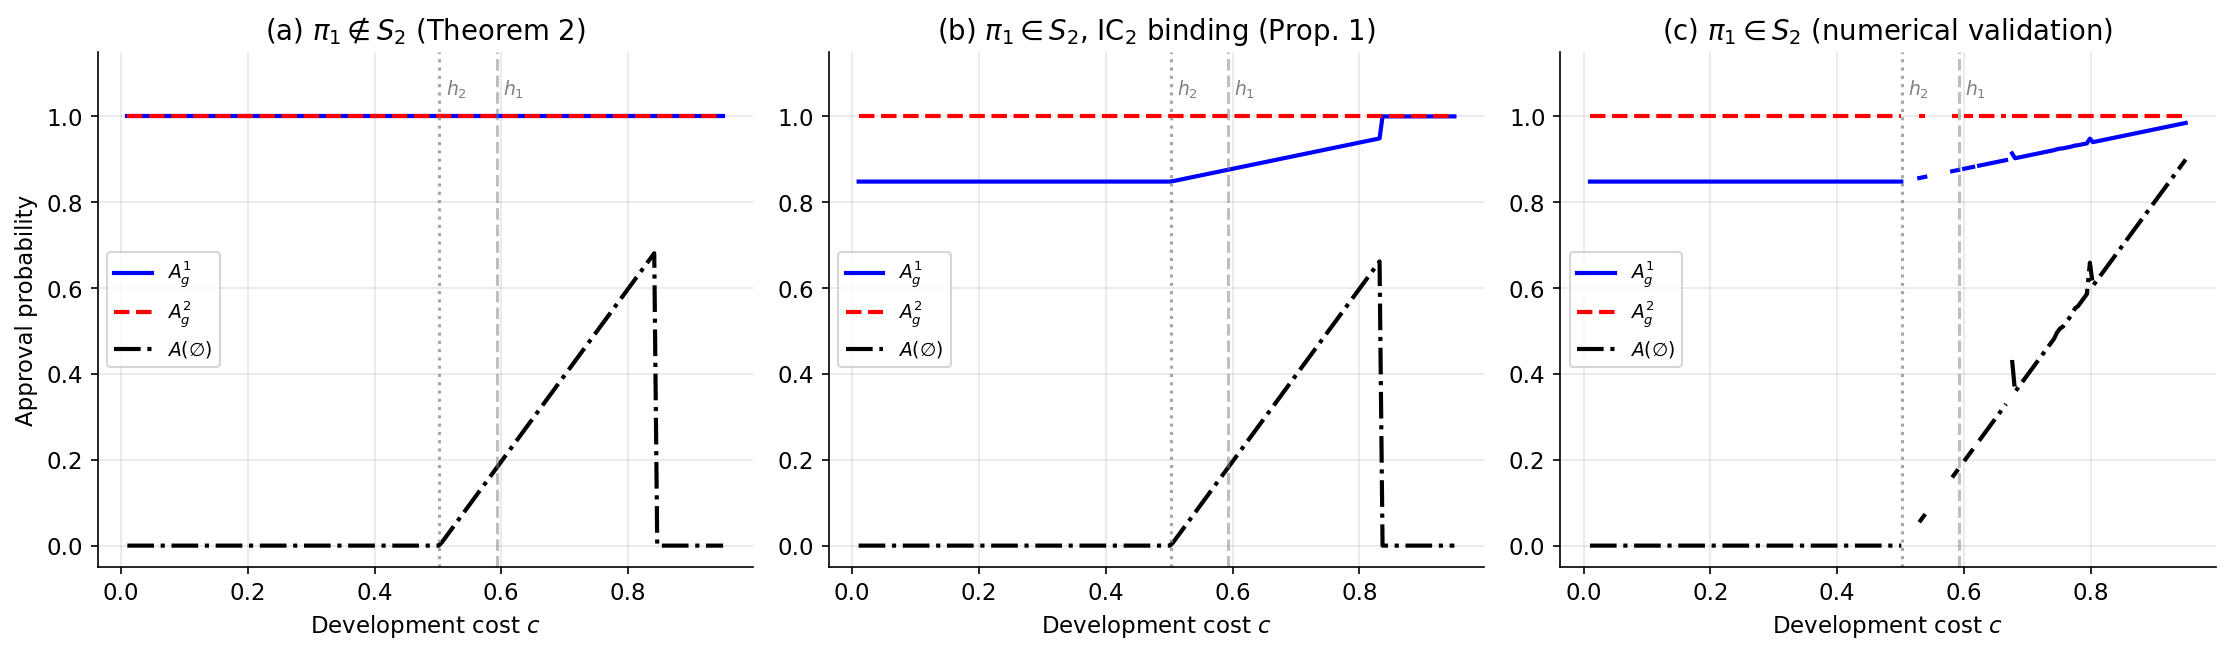
\includegraphics[width=\textwidth]{fig1_approval_vs_cost.png}
  \caption{Optimal approval probabilities as a function of
    development cost~$c$. Panel~(a): $\pi_1 \notin S_2$
    (closed-form, Theorem~\ref{thm:with_IR}). Panel~(b):
    $\pi_1 \in S_2$, both ICs binding
    (Proposition~\ref{prop:both_IC}). Panel~(c): full
    numerical optimisation for validation. Vertical lines
    mark $c = h_2$ and $c = h_1$.}
  \label{fig:approval}
\end{figure}

Key observations:
\begin{enumerate}
  \item \textbf{Same $A(\emptyset)$, different $A_g^1$.}
    Both Cases~A and~B set $A(\emptyset) = \alpha^*$
    identically. The difference is entirely in $A_g^1$:
    Case~B distorts it downward from 1 to
    $\approx 0.85$ (Figure~\ref{fig:approval}, panels a
    vs.~b).

  \item \textbf{Numerical validation.}
    The scipy solution (panel~c) matches
    Proposition~\ref{prop:both_IC} to three decimal places,
    confirming the semi-closed-form.

  \item \textbf{Welfare ordering.}
    Figure~\ref{fig:payoff} shows $V_A > V_B$ for all $c$:
    the IC$_2$ constraint strictly reduces the FDA's payoff.
    The welfare loss from the binding IC$_2$ constraint is
    $t \, \Delta_g(\pi_1)(1-A_g^1)$.
\end{enumerate}

\begin{figure}[htbp]
  \centering
  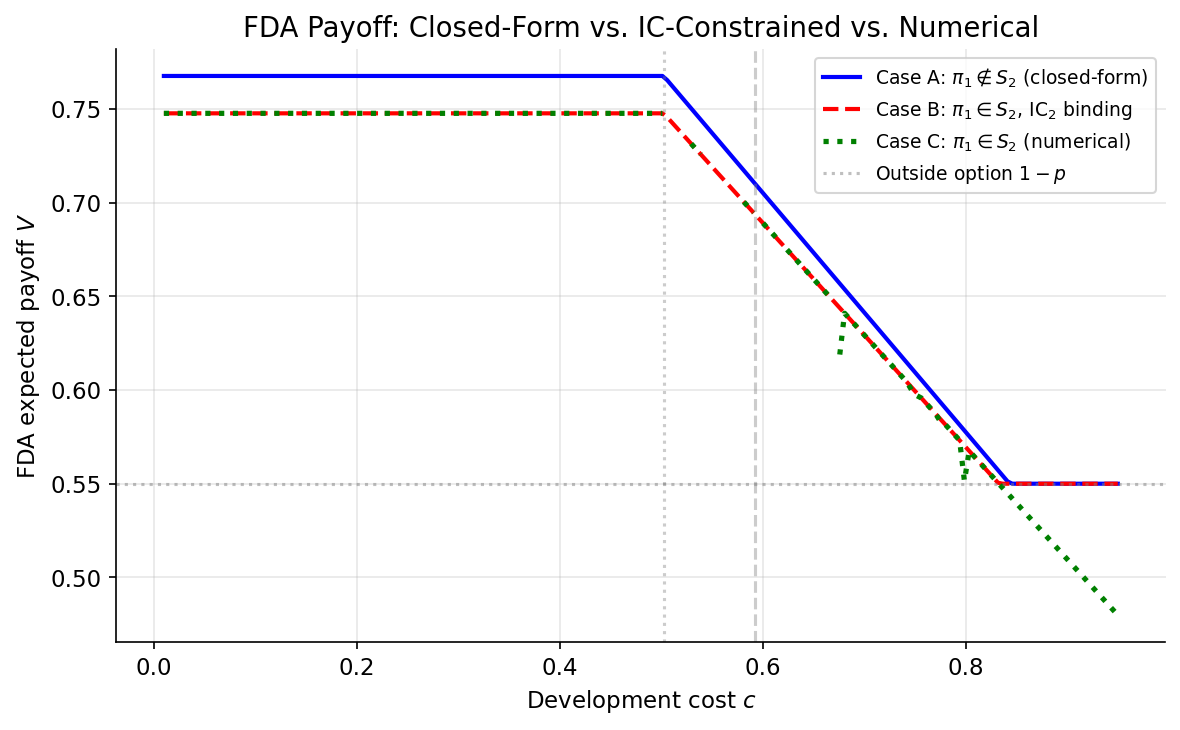
\includegraphics[width=0.7\textwidth]{fig2_fda_payoff.png}
  \caption{FDA expected payoff across regimes. The gap
    between Cases~A and~B measures the welfare cost of the
    IC$_2$ constraint. The horizontal line is the outside
    option $1-p$.}
  \label{fig:payoff}
\end{figure}


% ============================================================
\section{Summary of Results}
\label{sec:summary}
% ============================================================

\begin{center}
\renewcommand{\arraystretch}{1.3}
\begin{tabular}{@{}lccc@{}}
\toprule
 & $c \leq h_2$ & $c \in (h_2, c^*)$ & $c \geq c^*$ \\
\midrule
$A(\emptyset)$ & $0$ & $\alpha^* > 0$ & $0$ \\
Cherry-picking & irrelevant & endogenous & irrelevant \\
Equivalent to Min? & yes & no & yes \\
Welfare cost & $0$ & $t|\Delta_b(\pi_1)|\alpha^*$ & $0$ \\
\midrule
IC$_2$ distortion &
  $A_g^1 = h_2/h_1 < 1$ &
  $A_g^1 = \alpha^*(1{-}h_2/h_1) + h_2/h_1$ &
  --- \\
\bottomrule
\end{tabular}
\end{center}

The bottom row applies only when $\pi_1 \in S_2$; otherwise
$A_g^1 = 1$ throughout.


% ============================================================
\section{Discussion}
\label{sec:discussion}
% ============================================================

Two policy implications follow from the analysis. First,
mandatory trial pre-registration restores the FDA's ability
to target subsidies. When the experiment $\pi$ is observable
even if the firm omits results, the approval probability for
no-evidence applications becomes experiment-specific:
$A(\emptyset) \to A(\pi, \emptyset)$, analogous to Min's
type-specific $A_b^i$. The pooling constraint is broken and
its welfare cost is eliminated. Second, government subsidies
or tax credits that lower the development cost $c$ can remove
the need for $A(\emptyset) > 0$ entirely, moving the economy
from the participation-constrained regime to the
unconstrained one. This is more efficient than tolerating
cherry-picking.

Several limitations deserve mention. Joint optimisation over
experiments \emph{and} approval probabilities with both IC
and IR constraints active is a higher-dimensional problem
that does not admit a clean closed form. The numerical
methods of Section~\ref{sec:numerical} handle the case of
fixed experiments; extending the analysis to endogenous
experiment choice remains an open direction. Additionally,
Min's sufficient conditions for favorite experiments and
ex~post optimality (Propositions~4--5 in the original paper)
have not been extended to the participation-constrained
setting, and doing so is non-trivial.


% ============================================================
\section*{References}
% ============================================================

\begin{thebibliography}{99}

\bibitem[AllTrials(2013)]{alltrials2013}
AllTrials Campaign (2013).
\emph{All Trials Registered, All Results Reported}.
\url{http://www.alltrials.net}.

\bibitem[De~Angelis et~al.(2004)]{deangelis2004}
De~Angelis, C.~D., Drazen, J.~M., Ehringhaus, S., et~al.
  (2004).
Clinical trial registration: a statement from the
  International Committee of Medical Journal Editors.
\emph{New England Journal of Medicine}, 351(12), 1250--1251.

\bibitem[Maskin and Riley(1984)]{maskinriley1984}
Maskin, E. and Riley, J. (1984).
Monopoly with incomplete information.
\emph{RAND Journal of Economics}, 15(2), 171--196.

\bibitem[Min(2023)]{min2023}
Min, D. (2023).
Screening for experiments.
\emph{Games and Economic Behavior}, 142, 898--920.

\bibitem[Mussa and Rosen(1978)]{mussarosen1978}
Mussa, M. and Rosen, S. (1978).
Monopoly and product quality.
\emph{Journal of Economic Theory}, 18(2), 301--317.

\bibitem[Turner et~al.(2008)]{turner2008}
Turner, E.~H., Matthews, A.~M., Linardatos, E., Tell,
  R.~A., and Rosenthal, R. (2008).
Selective publication of antidepressant trials and its
  influence on apparent efficacy.
\emph{New England Journal of Medicine}, 358(3), 252--260.

\end{thebibliography}


\end{document}
